\documentclass[12pt]{beamer}
\usetheme{CambridgeUS}
\usepackage[utf8]{inputenc}
\usepackage{amsmath}
\usepackage{amsfonts}
\usepackage{amssymb}
\author{Witten and Tibshirani}
\title{A Framework for Feature Selection in Clustering}
%\setbeamercovered{transparent} 
%\setbeamertemplate{navigation symbols}{} 
%\logo{} 
%\institute{} 
%\date{} 
%\subject{} 
\begin{document}

\begin{frame}
\titlepage
\end{frame}

%\begin{frame}
%\tableofcontents
%\end{frame}

\begin{frame}{Introduction}
\begin{itemize}
\item Let $X$ denotes an $n\times p$ data matrix, with $n$ observations and $p$ features.
\item Suppose that we wish to cluster the observations, and
we suspect that the true underlying clusters differ only with respect
to some of the features.
\item We propose a method for sparse
clustering, which allows us to group the observations using only
an adaptively chosen subset of the features.
\end{itemize}
\end{frame}

\begin{frame}{Clustering}
\begin{itemize}
\item Kmeans
\item Hierarchical clustering
\item GMM, DBSCAN,manifold learning(t-SNE)
\end{itemize}
\end{frame}

\begin{frame}{Dissimilarity}
\begin{itemize}
\item  Clustering methods require some concept of the dissimilarity(or distance) between pairs of observations.
\item Throughout this paper,
we will assume that $d$ is additive in the features.That is
$$
d(x_i,x_{i^{'}})=\sum_{j=1}^p d_{i,i^{'},j}.
$$
\item In this paper, we take $d$ to be squared Euclidean distance, but other dissimilarity measures are possible.
\end{itemize}
\end{frame}

\section{Past Work on Sparse Clustering}
\begin{frame}{Matrix decomposition}
One way to reduce the dimensionality of the data before clustering
is by performing a matrix decomposition.
\begin{itemize}
\item One can approximate the $n \times p$ data matrix $X$ as $X\approx AB$ where $A$ is a $n \times q$ matrix and $B$is a $q\times p$ matrix, $q\ll p$.
\item For instance, PCA, Non-negative Matrix Factorization. 
\end{itemize}
\end{frame}

\begin{frame}{Matrix decomposition}
However, these approaches have a number of drawbacks.
\begin{itemize}
\item The resulting clustering is not sparse in the features.
\item There is no guarantee that A contains the signal
that one is interested in detecting via clustering. 
\item For example, the principal components with largest eigenvalues
do not necessarily provide the best separation between subgroups.
\end{itemize}
\end{frame}

\begin{frame}{GMM}
\begin{itemize}
\item One can model the rows of X as independent
multivariate observations drawn from a mixture model
with K components
\item usually a mixture of Gaussians is used.That is, given the data, the log-likelihood is
\end{itemize}
$$
\sum_{i=1}^{n} \log \left[\sum_{k=1}^{K} \pi_{k} f_{k}\left(\mathbf{X}_{i} ; \mu_{k}, \mathbf{\Sigma}_{k}\right)\right],
$$
where $f_k$ is a Gaussian density parametrized by its mean $\mu_k$ and covariance matrix $\Sigma_k$. The EM algorithm can be used to fit his model.
\end{frame}

\begin{frame}{feature selection in GMM}
We can maximize the penalized log-likelihood
$$
\sum_{i=1}^{n} \log \left[\sum_{k=1}^{K} \pi_{k} f_{k}\left(\mathbf{X}_{i} ; \mu_{k}, \mathbf{\Sigma}_{k}\right)\right]-\lambda \sum_{k=1}^{K} \sum_{j=1}^{p}\left|\mu_{k j}\right|,
$$
where $\Sigma_{1}=\cdots=\Sigma_{K}$ is taken to be a diagonal matrix.
\begin{itemize}
\item The $L_1$ penalty is applied to the elements of $\mu_k$.
\item Some of the elements of $\mu_k$ will be exactly zero.
\item If, for some variable $j$, $\mu_{kj}=0$ for all $k=1,\dots,K$, then the resulting clustering
will not involve feature $j$.
\end{itemize}
\end{frame}


\begin{frame}{COSA}
\begin{itemize}
\item Friedman and Meulman (2004) propose clustering objects on
subsets of attributes (COSA).
\item Let $C_k$ denote the indices of the
observations in the $k$th of the $K$ clusters. Then, the COSA criterion is
$$
\operatorname{minimize}_{C_{1}, \ldots, C_{K}, \mathbf{w}}\left\{\sum_{k=1}^{K} a_{k} \sum_{i, i^{\prime} \in C_{k}} \sum_{j=1}^{p}\left(w_{j} d_{i, i^{\prime}, j}+\lambda w_{j} \log w_{j}\right)\right\}
$$
$$
\text { subject to } \sum_{i=1}^{p} w_{j}=1, \quad w_{j} \geq 0 \quad \forall j.
$$
Here, $a_k$ is some function of the number of elements in cluster $k$, $w\in \mathbb{R}^p$ a vector of feature weights.
\end{itemize}
\end{frame}

\begin{frame}{COSA}
\begin{itemize}
\item  It can be seen that this criterion is related to
a weighted version of K-means clustering.
\item Unfortunately, this
proposal does not truly result in a sparse clustering, since all
variables have nonzero weights for $\lambda>0$.
\item An extension of (3)
is proposed in order to generalize the method to other types of
clustering, such as hierarchical clustering.
\end{itemize}
\end{frame}

\section{The Proposed Sparse Clustering Framework}
\begin{frame}
Let $\mathbf{X}_{j}\in \mathbb{R}^n$ denote feature $j$. Many clustering methods can be expressed as an optimization problem of the form 
$$
\underset{\mathbf{\Theta} \in D}{\operatorname{maximize}}\left\{\sum_{j=1}^{p} f_{j}\left(\mathbf{X}_{j}, \mathbf{\Theta}\right)\right\}
$$
where $f_j(\mathbf{X}_{j},\mathbf{\Theta})$ is some function that involves only the $j$th feature of the data.

K-means and hierarchical clustering are two such examples, as
we show in the next few sections. 
\end{frame}

\begin{frame}
We define sparse clustering as the solution to the problem


\begin{equation}\tag{5}
\begin{array}{c}
\operatorname{maximize}_{\mathbf{w} ; \mathbf{\Theta} \in D}\left\{\sum_{j=1}^{p} w_{j} f_{j}\left(\mathbf{X}_{j}, \mathbf{\Theta}\right)\right\} \\
\text { subject to }\|\mathbf{w}\|^{2} \leq 1, \quad\|\mathbf{w}\|_{1} \leq s ,\\
w_{j} \geq 0 \quad \forall j ,
\end{array}
\end{equation}
where $w_j$ is a weight corresponding to feature $j$ and $s$ is a tuning parameter, $1\le s \le \sqrt{p}$.
\end{frame}

\begin{frame}{Optimization}
We optimize (5) using an iterative algorithm:
\begin{itemize}
\item holding $\mathbf{w}$ fixed, we optimize (5) with respect to $\mathbf{\Theta}$
\item holding $\mathbf{\Theta}$ fixed, we optimize (5) with respect to $\mathbf{w}$.
\end{itemize}
In general, we do not achieve a global optimum of (5) using this iterative approach.

However, we are guaranteed that each iteration increases the objective function.
\end{frame}

\begin{frame}{Optimization}
To optimize (5) with respect to $\mathbf{w}$ with $\mathbf{\Theta}$ held fixed, we note that the problem can be rewritten as
\begin{equation}\tag{6}
\begin{array}{cl}
\underset{\mathbf{w}}{\operatorname{maximize}}\left\{\mathbf{w}^{T} \mathbf{a}\right\} \\
\text { subject to } & \|\mathbf{w}\|^{2} \leq 1, \quad\|\mathbf{w}\|_{1} \leq s \\
 & w_{j} \geq 0 \qquad \forall j,
\end{array}
\end{equation}
where $a_j=f_j(\mathbf{X}_j,\mathbf{\Theta})$. 
\end{frame}

\begin{frame}{Optimization}
This can be solved by KKT conditions.
\end{frame}

\section{Sparse K–means Clustering}
\begin{frame}{K-means}
K-means clustering minimizes the within-cluster sum of
squares (WCSS). That is, it seeks to partition the n observations
into K sets, or clusters, such that the WCSS
$$
\sum_{k=1}^{K} \frac{1}{n_{k}} \sum_{i, i^{\prime} \in C_{k}} \sum_{j=1}^{p} d_{i, i^{\prime}, j}
$$
is minimal, where $n_k$ is the number of observations in cluster $k$.
Note that if we define the
between-cluster sum of squares (BCSS) as
$$
\sum_{j=1}^{p}\left(\frac{1}{n} \sum_{i=1}^{n} \sum_{i^{\prime}=1}^{n} d_{i, i^{\prime}, j}-\sum_{k=1}^{K} \frac{1}{n_{k}} \sum_{i, i^{\prime} \in C_{k}} d_{i, i^{\prime}, j}\right),
$$
then minimizing the WCSS is equivalent to maximizing the
BCSS.
\end{frame}

\begin{frame}{Sparse K-means}
One could try to develop a method for sparse K-means clustering
by optimizing a weighted WCSS, subject to constraints
on the weights: that is,
$$
\begin{array}{c}
\left.\operatorname{maximize}_{C_{1}, \ldots, C_{K}, \mathbf{w}}\left\{\sum_{j=1}^{p} w_{j}\left(-\sum_{k=1}^{K} \frac{1}{n_{k}} \sum_{i, i^{\prime} \in C_{k}} d_{i, i^{\prime}, j}\right)\right\}\right\} \\
\text { subject to }\|\mathbf{w}\|^{2} \leq 1, \quad\|\mathbf{w}\|_{1} \leq s \\
w_{j} \geq 0 \quad \forall j.
\end{array}
$$
Since each element of the
weighted sum is negative, the maximum occurs when all
weights are zero, regardless of the value of s. This is not an interesting question.
\end{frame}

\begin{frame}{Sparse K-Means}
We instead maximize a weighted BCSS,
subject to constraints on the weights. Our sparse K-means clustering
criterion is as follows:
$$
\operatorname{maximize}_{C_{1}, \ldots, C_{K}, \mathbf{w}}\left\{\sum_{j=1}^{p} w_{j}\left(\frac{1}{n} \sum_{i=1}^{n} \sum_{i=1}^{n} d_{i, i^{\prime}, j}-\sum_{k=1}^{K} \frac{1}{n_{k}} \sum_{i, i^{\prime} \in C_{k}} d_{i, i^{\prime}, j}\right)\right\}
$$
$$
\begin{array}{ll}
\text { subject to } & \|\mathbf{w}\|^{2} \leq 1, \quad\|\mathbf{w}\|_{1} \leq s \\
& w_{j} \geq 0 \quad \forall j.
\end{array}
$$
The weights will be sparse for an appropriate choice of the tuning
parameter $s$, which should satisfy $1\le s \le \sqrt{p}$.
\end{frame}

\begin{frame}{Algorithm for Sparse K-Means clustering}
\begin{itemize}
\item Initialize $\mathbf{w}$ as $w_1=\dots=w_p=1/\sqrt{p}$.
\item Iterate until convergence:
\begin{itemize}
\item Holding $w$ fixed, optimize with respect to $C_1,\dots,C_K$.
\item Holding $C_1,\dots,C_K$ fixed, optimize with respect to $\mathbf{w}$.
\end{itemize}
\item The clusters are given by $C_1,\dots,C_K$, and the feature
weights corresponding to this clustering are given by $w_1,\dots,w_p$.
\end{itemize}
\end{frame}

\begin{frame}{Selection of Tuning Parameter}
\begin{itemize}
\item The sparse K-means clustering algorithm has one tuning parameter $w$.
\item We assume that K, the number of clusters, is fixed.
\item Note that
one cannot simply select s to maximize the objective function
, since as $s$ is increased, the objective will increase as
well.
\item Instead, we apply a permutation approach that is closely
related to the gap statistic.
\end{itemize}
\end{frame}

\begin{frame}{Algorithm to select tuning parameter s}
\begin{itemize}
\item Obtain permuted datasets $\mathbf{X}_1,\dots,\mathbf{X}_B$ by independently
permuting the observations within each feature.
\item For each candidate tuning parameter value s:
\begin{itemize}
\item Compute the objective function $$O(s)=\sum_{i} w_{j}(\frac{1}{n} \sum_{i=1}^{n} \sum_{i^{\prime}=1}^{n} d_{i, i^{\prime}, j}-\sum_{k=1}^{K} \frac{1}{n_{k}} \sum_{i, i^{\prime} \in C_{k}} d_{i, i^{\prime}, j})$$
\item For $b=1,2,\dots,B$, compute $O_b(s)$.
\item Calculate $Gap(s)=\log(O(s))-\dfrac{1}{B}\sum_{b=1}^B \log(O_B(s))$.
\end{itemize}
\item Choose $s^{*}$ corresponding to the largest value of $Gap(s)$.
\end{itemize}
\end{frame}

\begin{frame}{Tuning parameter selection}
\begin{itemize}
\item Note that while there may be strong correlations between the
features in the original data $\mathbf{X}$, the features in the permuted
datasets $\mathbf{X}_1, . . . ,\mathbf{X}_B$ are uncorrelated with each other. 
\item The gap
statistic measures the strength of the clustering obtained on the
real data relative to the clustering obtained on null data that does
not contain subgroups.
\item  The optimal tuning parameter value occurs
when this quantity is greatest.
\end{itemize}
\end{frame}

\begin{frame}{Tuning parameter selection}
We apply this method to a simple example with 6
equally sized classes, where $n = 120, p = 2000, and 200$ features
differ between classes.

In the figure we have used the
classification error rate (CER) for two partitions of a set of n
observations.
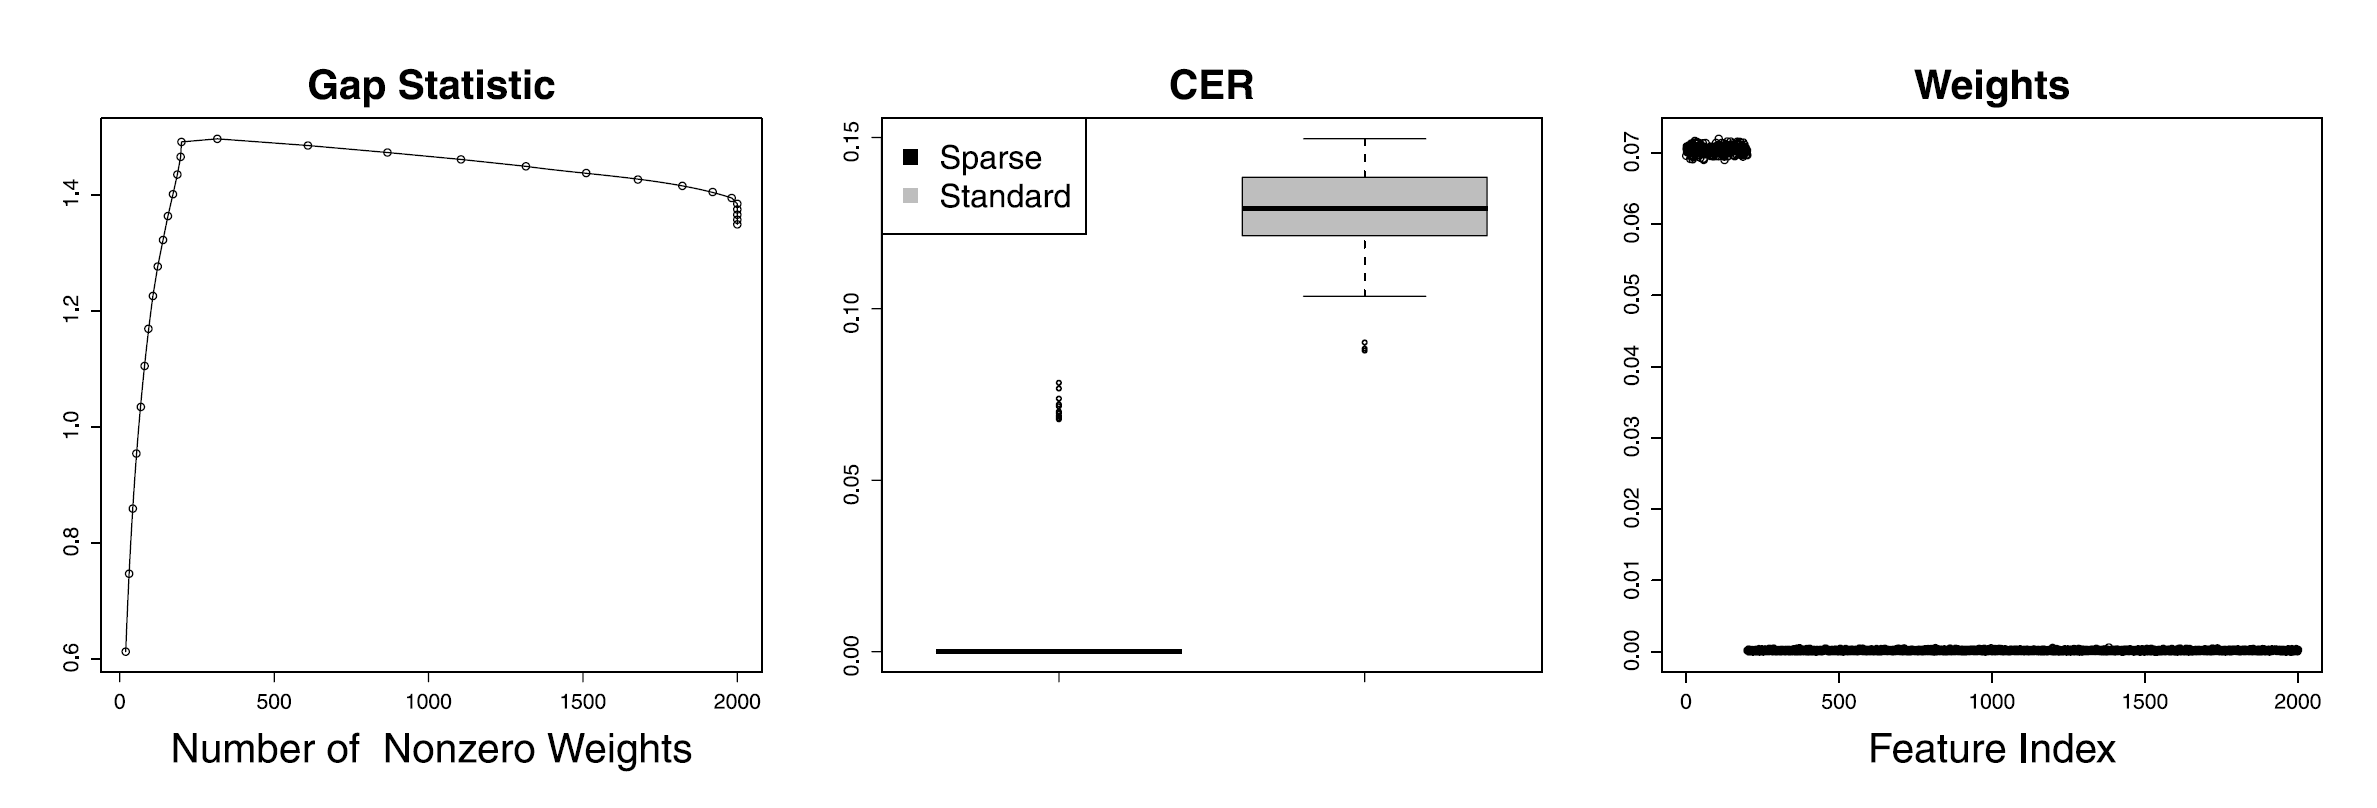
\includegraphics[scale=0.5]{fig1.png} 
\end{frame}

\begin{frame}{A Comparison of Sparse and Standard
K-Means}
\begin{itemize}
\item We compare the performances of standard and
sparse K-means in a simulation study where $q=50$ features differ between $K=3$ classes.
\item $X_{ij}\sim N(\mu_{ij},1)$ independent; $\mu_{i j}=\mu\left(1_{i \in C_{1}, j \leq q}-1_{i \in C_{2}, j \leq q}\right)$.
\item Datasets were generated with
various values of $\mu$ and $p$, with 20 observations per class.
\end{itemize}
\end{frame}


\begin{frame}{A Comparison of Sparse and Standard
K-Means}
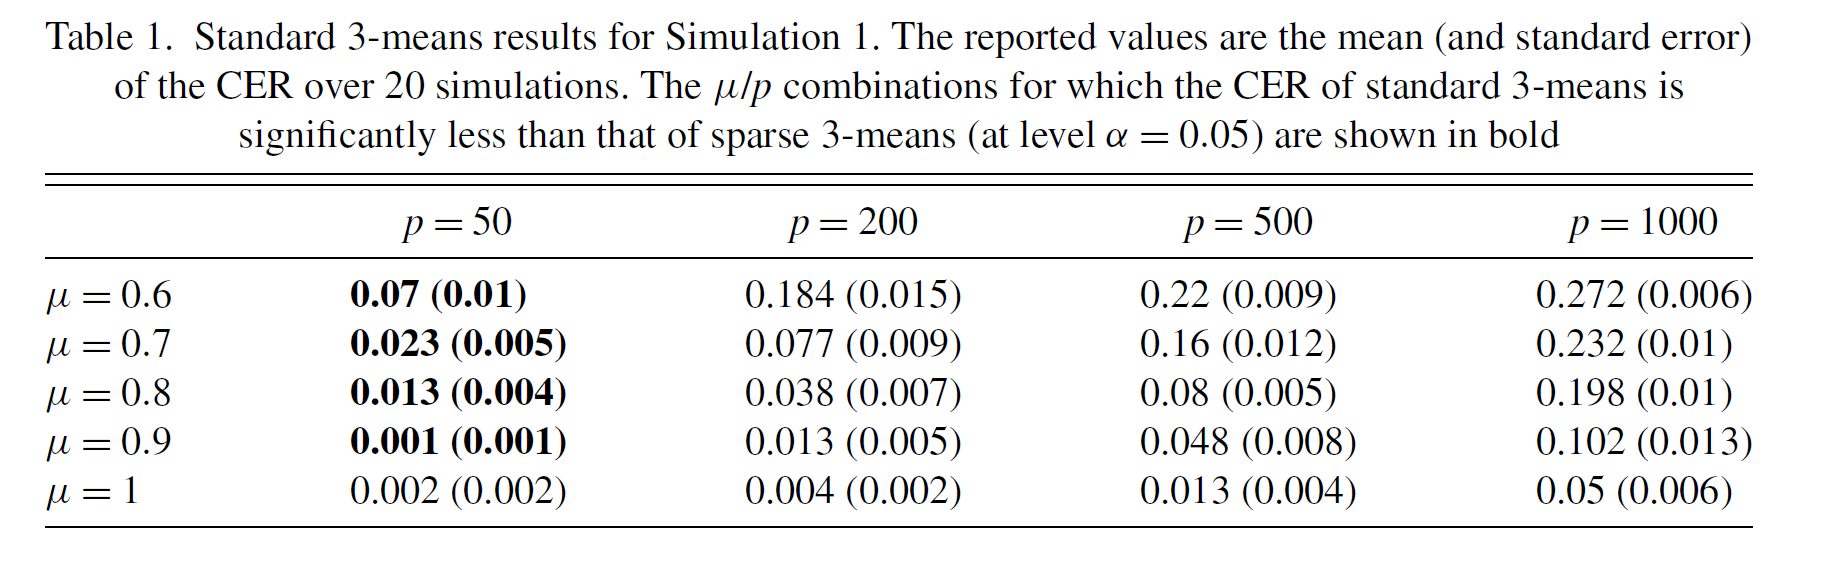
\includegraphics[scale=0.6]{fig2.png} 
\end{frame}

\begin{frame}{A Comparison of Sparse and Standard
K-Means}
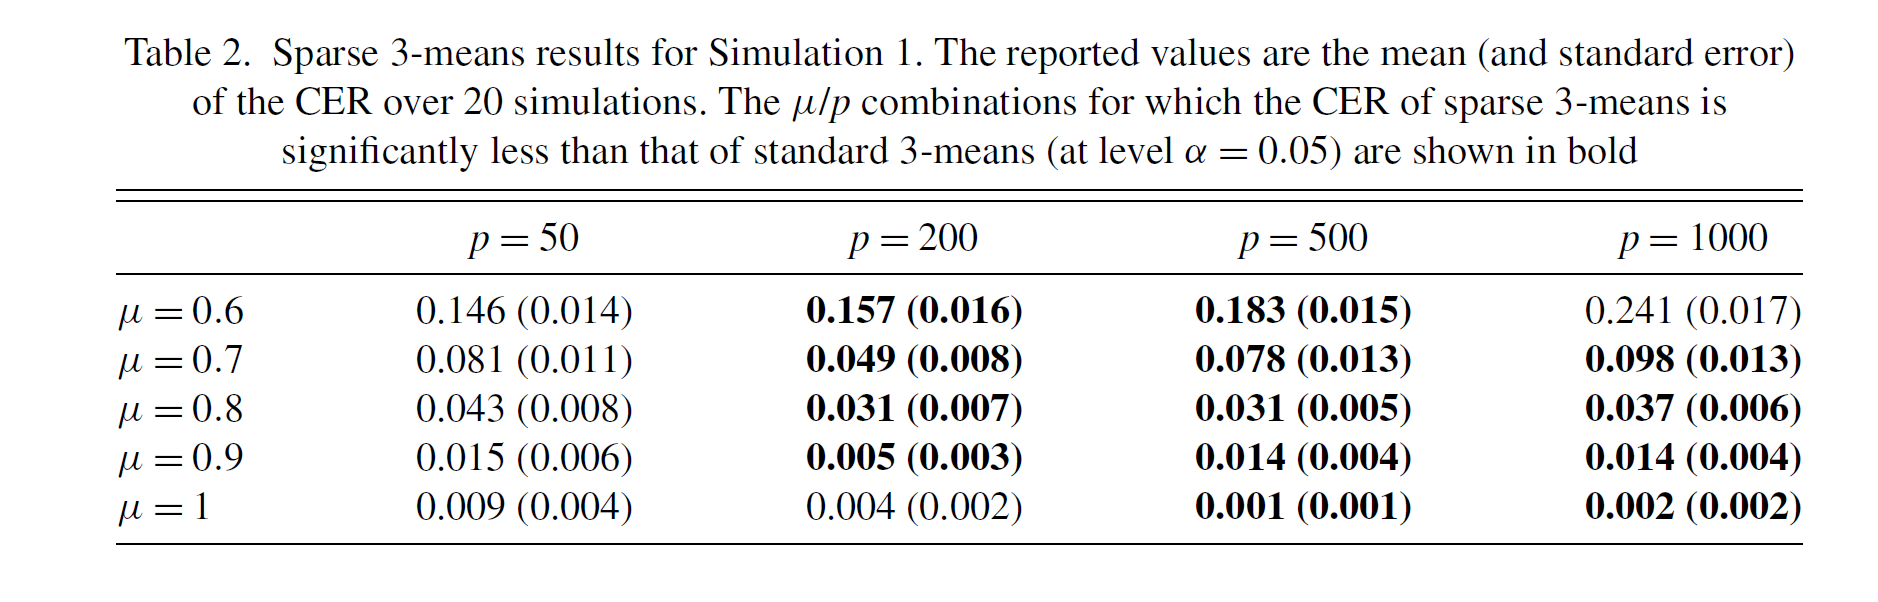
\includegraphics[scale=0.6]{fig3.png} 
\end{frame}

\begin{frame}{A Comparison of Sparse and Standard
K-Means}
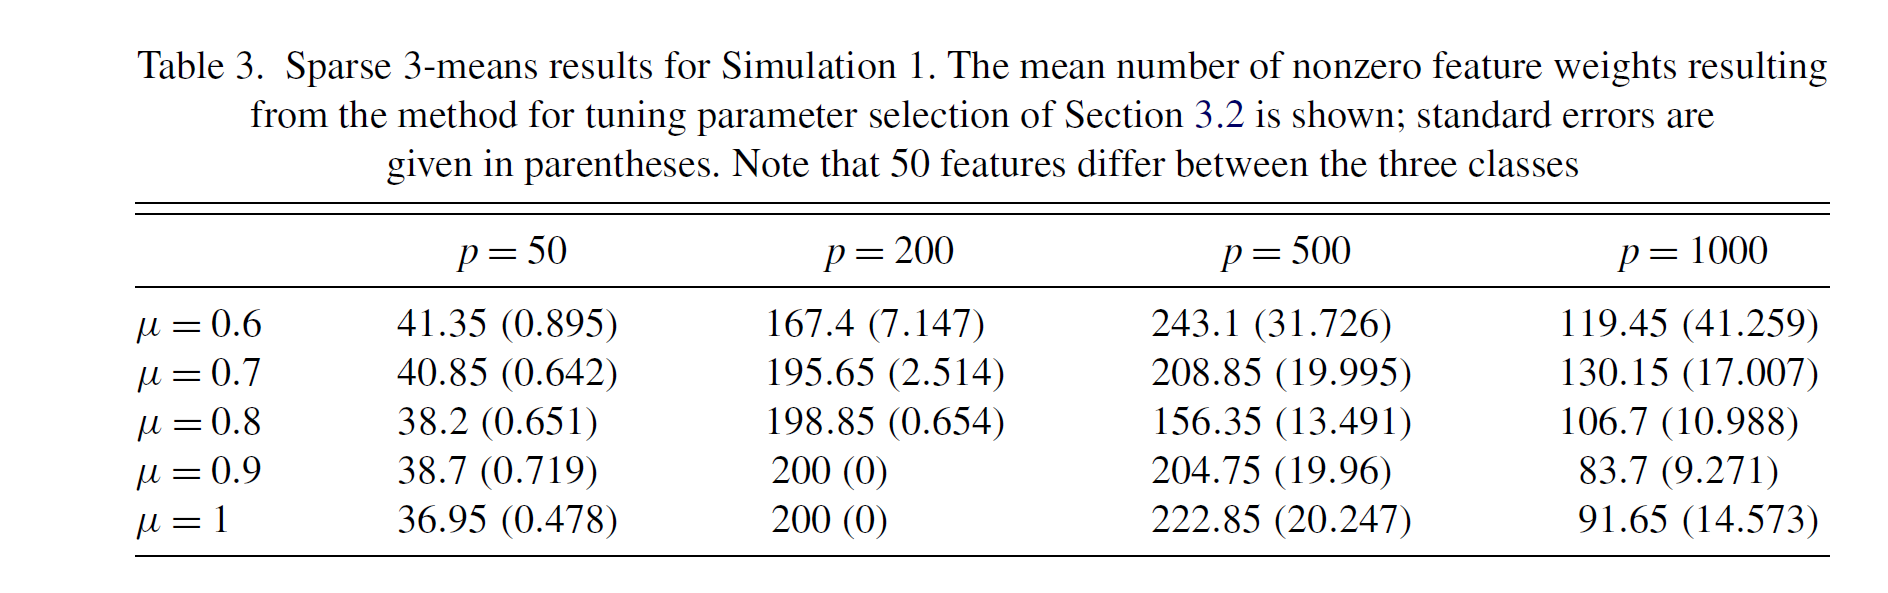
\includegraphics[scale=0.6]{fig4.png} 
\end{frame}

\begin{frame}{A Comparison With Other Approaches}
We compare the performance of sparse K-means to a number
of competitors:
\begin{itemize}
\item COSA
\item The model-based clustering approach of Raftery
and Dean(2006)
\item The penalized log-likelihood approach of Pan and Shen
(2007)
\item PCA followed by 3-means clustering.
\end{itemize}
\end{frame}

\begin{frame}{A Comparison With Other Approaches}
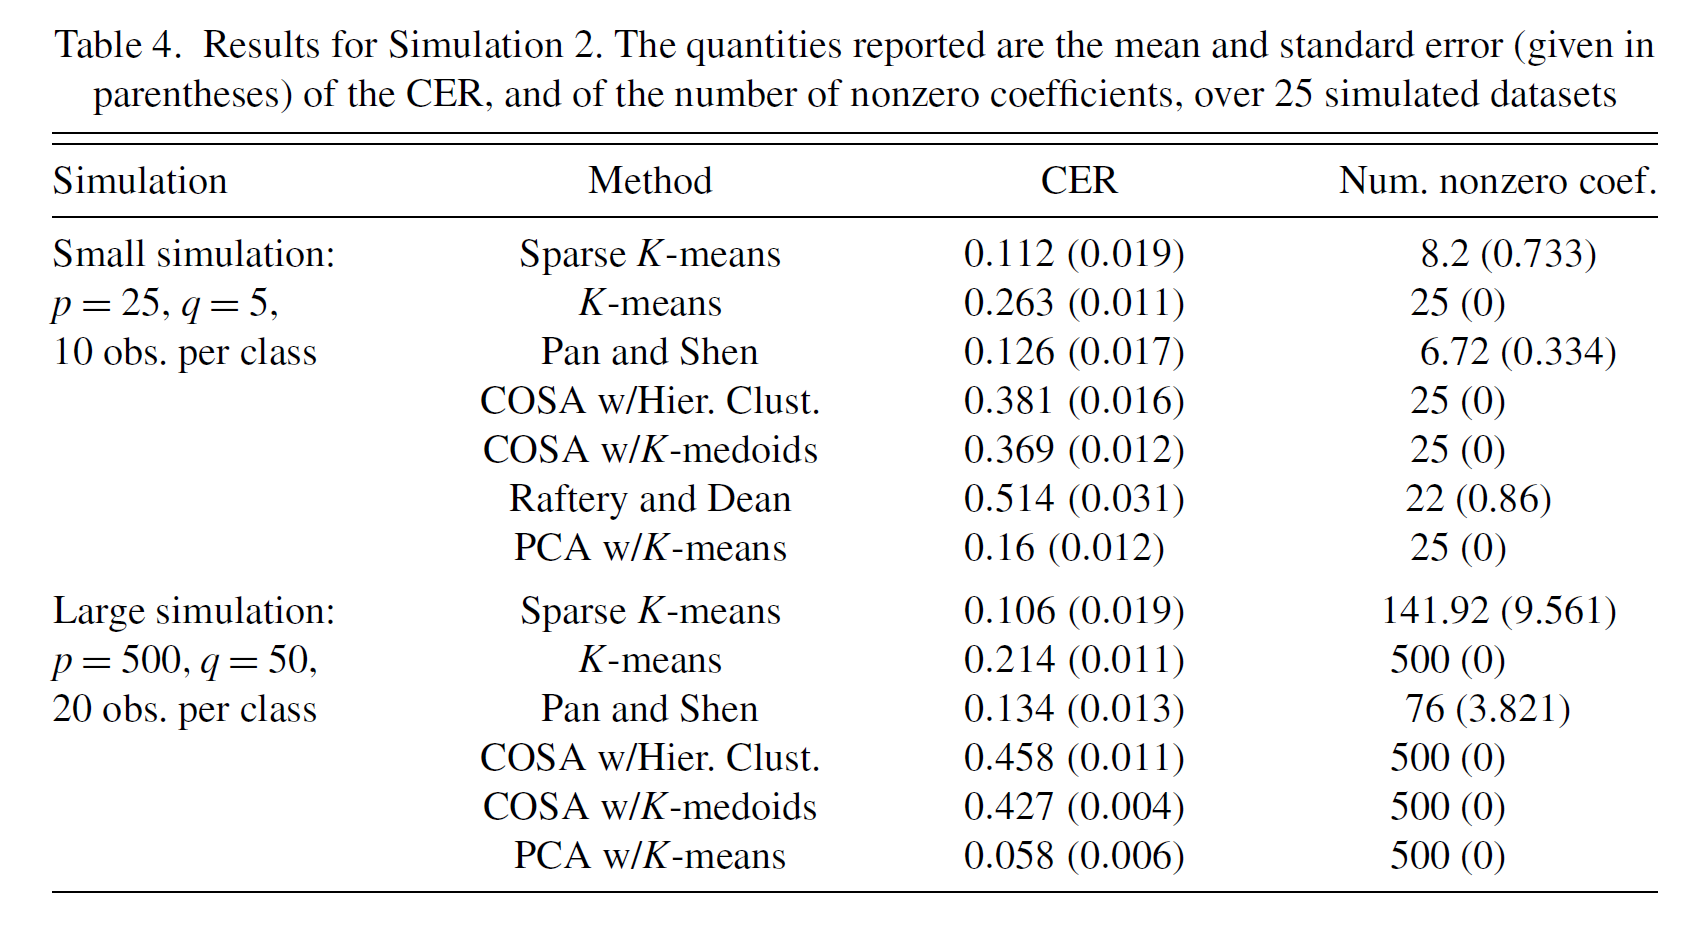
\includegraphics[scale=0.6]{fig5.png}
\end{frame}

\section{Sparse Hierarchical Clustering}
\begin{frame}{The Sparse Hierarchical Clustering Method}
\begin{itemize}
\item Note that hierarchical clustering takes as input a $n \times n$ dissimilarity matrix $U$.
\item The clustering can use any type of linkage—
complete, average, or single.
\item If $U$ s the overall dissimilarity
matrix $\{ \sum_{j} d_{i,i^{'},j}\}_{i,i^{'}}$,then standard hierarchical clustering results.
\item In this section, we cast the overall dissimilarity matrix $\{ \sum_{j} d_{i,i^{'},j}\}_{i,i^{'}}$ in the form (4), and then propose a criterion of
the form (5) that leads to a reweighted dissimilarity matrix that
is sparse in the features. 
\end{itemize}
\end{frame}

\begin{frame}{The Sparse Hierarchical Clustering Method}
Since scaling the dissimilarity matrix by a factor does not
affect the shape of the resulting dendrogram, we ignore proportionality
constants in the following discussion. Consider the
criterion
\begin{equation}\tag{14}
\begin{array}{c}
\underset{\mathbf{U}}{\operatorname{maximize}}\left\{\sum_{j} \sum_{i, i^{\prime}} d_{i, i^{\prime}, j} U_{i, i^{\prime}}\right\} \\
\text { subject to } \quad \sum U_{i, i^{\prime}}^{2} \leq 1.
\end{array}
\end{equation}
Let $U^*$ optimize (14). It is not hard to show that $U^{*}_{i,i^{'}}\propto \sum_{j} d_{i, i^{\prime}, j}$, and so performing hierarchical clustering on $U^*$ results in standard
hierarchical clustering.
\end{frame}


\begin{frame}{The Sparse Hierarchical Clustering Method}
we modify (14) by multiplying each
element of the summation over j by a weight wj, subject to constraints
on the weights:
$$
\underset{\mathbf{w}, \mathbf{U}}{\operatorname{maximize}}\left\{\sum_{j} w_{j} \sum_{i, i^{\prime}} d_{i, i^{\prime}, j} U_{i, i^{\prime}}\right\}
$$
\begin{equation}\tag{15}
\begin{array}{ll}
\text { subject to } & \sum_{i, i^{\prime}} U_{i, i^{\prime}}^{2} \leq 1, \quad\|\mathbf{w}\|^{2} \leq 1, \quad\|\mathbf{w}\|_{1} \leq s \\
& w_{j} \geq 0 \quad \forall j
\end{array}
\end{equation}
\end{frame}


\begin{frame}{Algorithm for sparse hierarchical clustering}
\begin{itemize}
\item Initialize $w$ as $w_1=\dots =w_p=1/\sqrt{p}$
\item Iterate until convergence:
\begin{itemize}
\item update $u$
\item update $w$
\end{itemize}
\item Rewrite $u$ as a $n \times n$ matrix $U$.
\item Perform hierarchical clustering on the $n \times n$ dissimilarity matrix $U$.
\end{itemize}
\end{frame}
\begin{frame}{Sparse Hierarchical clustering}
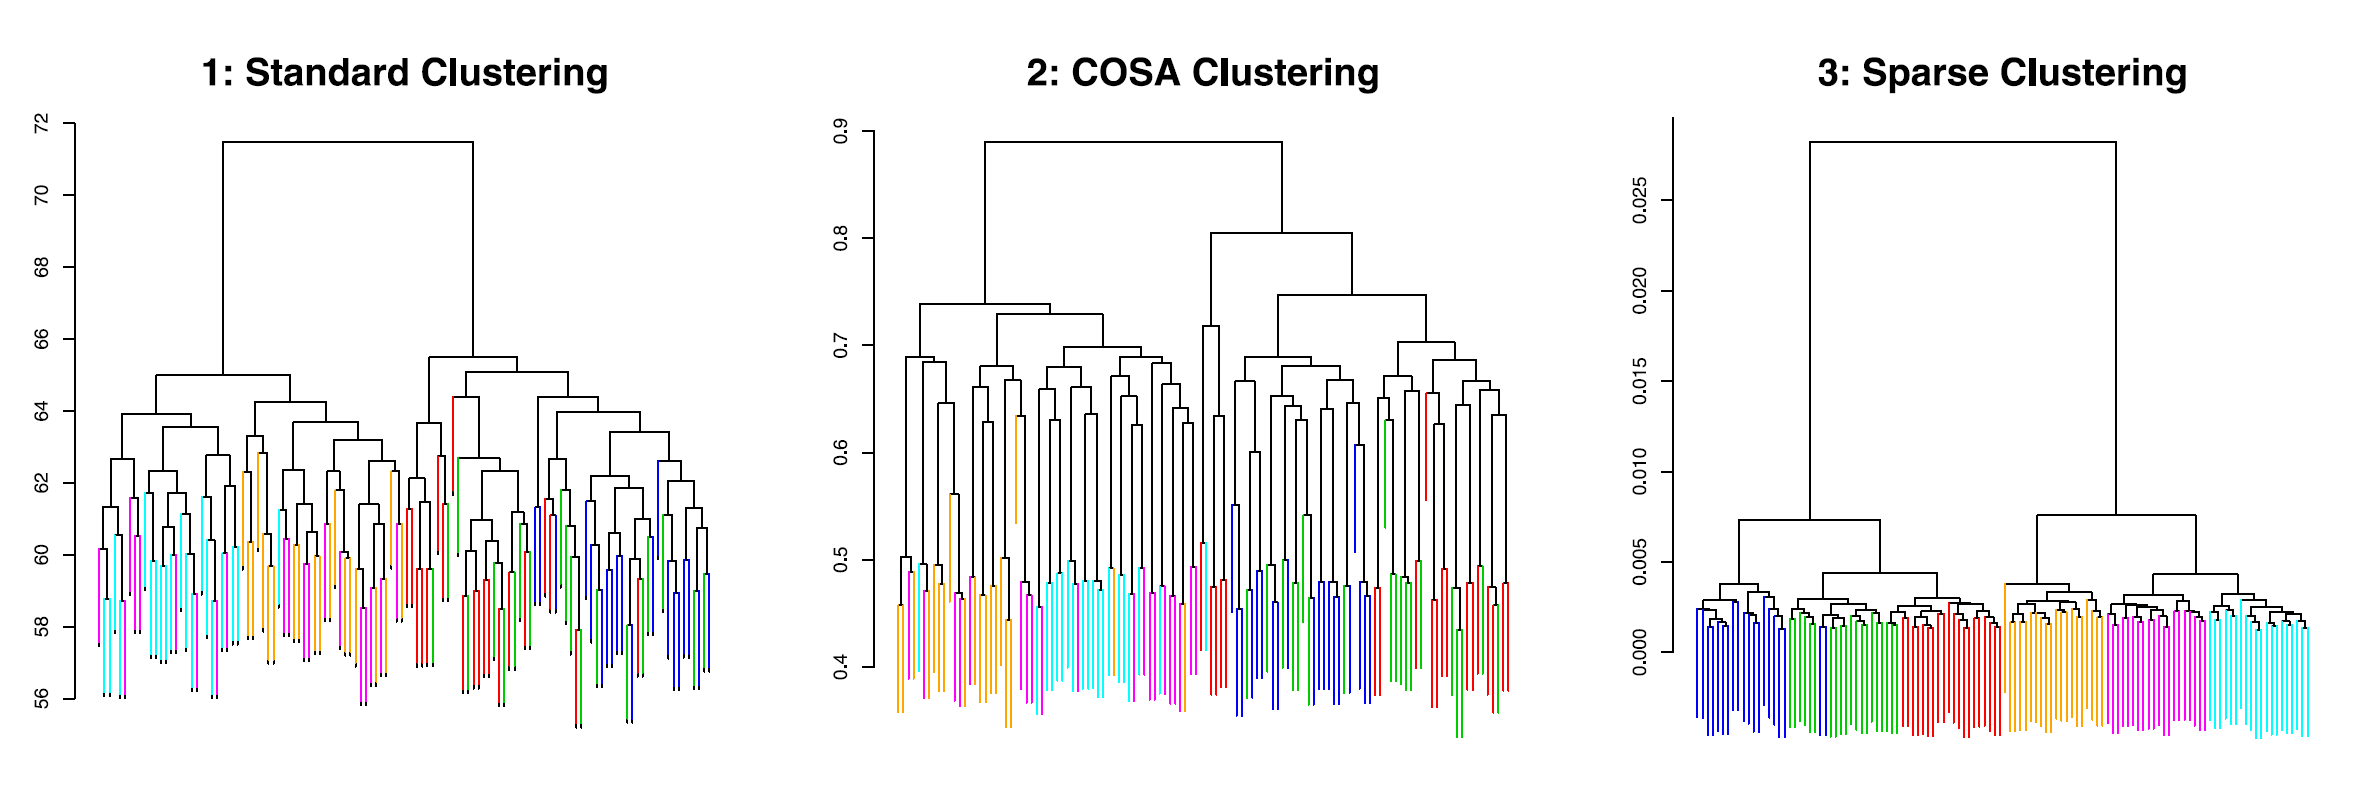
\includegraphics[scale=0.5]{fig6.png}
\end{frame}

\begin{frame}{Reanalysis of a breast cancer dataset}
We performed four versions of hierarchical
clustering with Eisen linkage on the 62 observations that were
assigned to the four classes:
\begin{itemize}
\item Sparse hierarchical clustering of all 1753 genes, with the
tuning parameter chosen to yield 496 nonzero genes
\item Standard hierarchical clustering using all 1753 genes.
\item Standard hierarchical clustering using the 496 genes with
highest marginal variance.
\item COSA hierarchical clustering using all 1753 genes.
\end{itemize}
\end{frame}

\begin{frame}{Reanalysis of a breast cancer dataset}
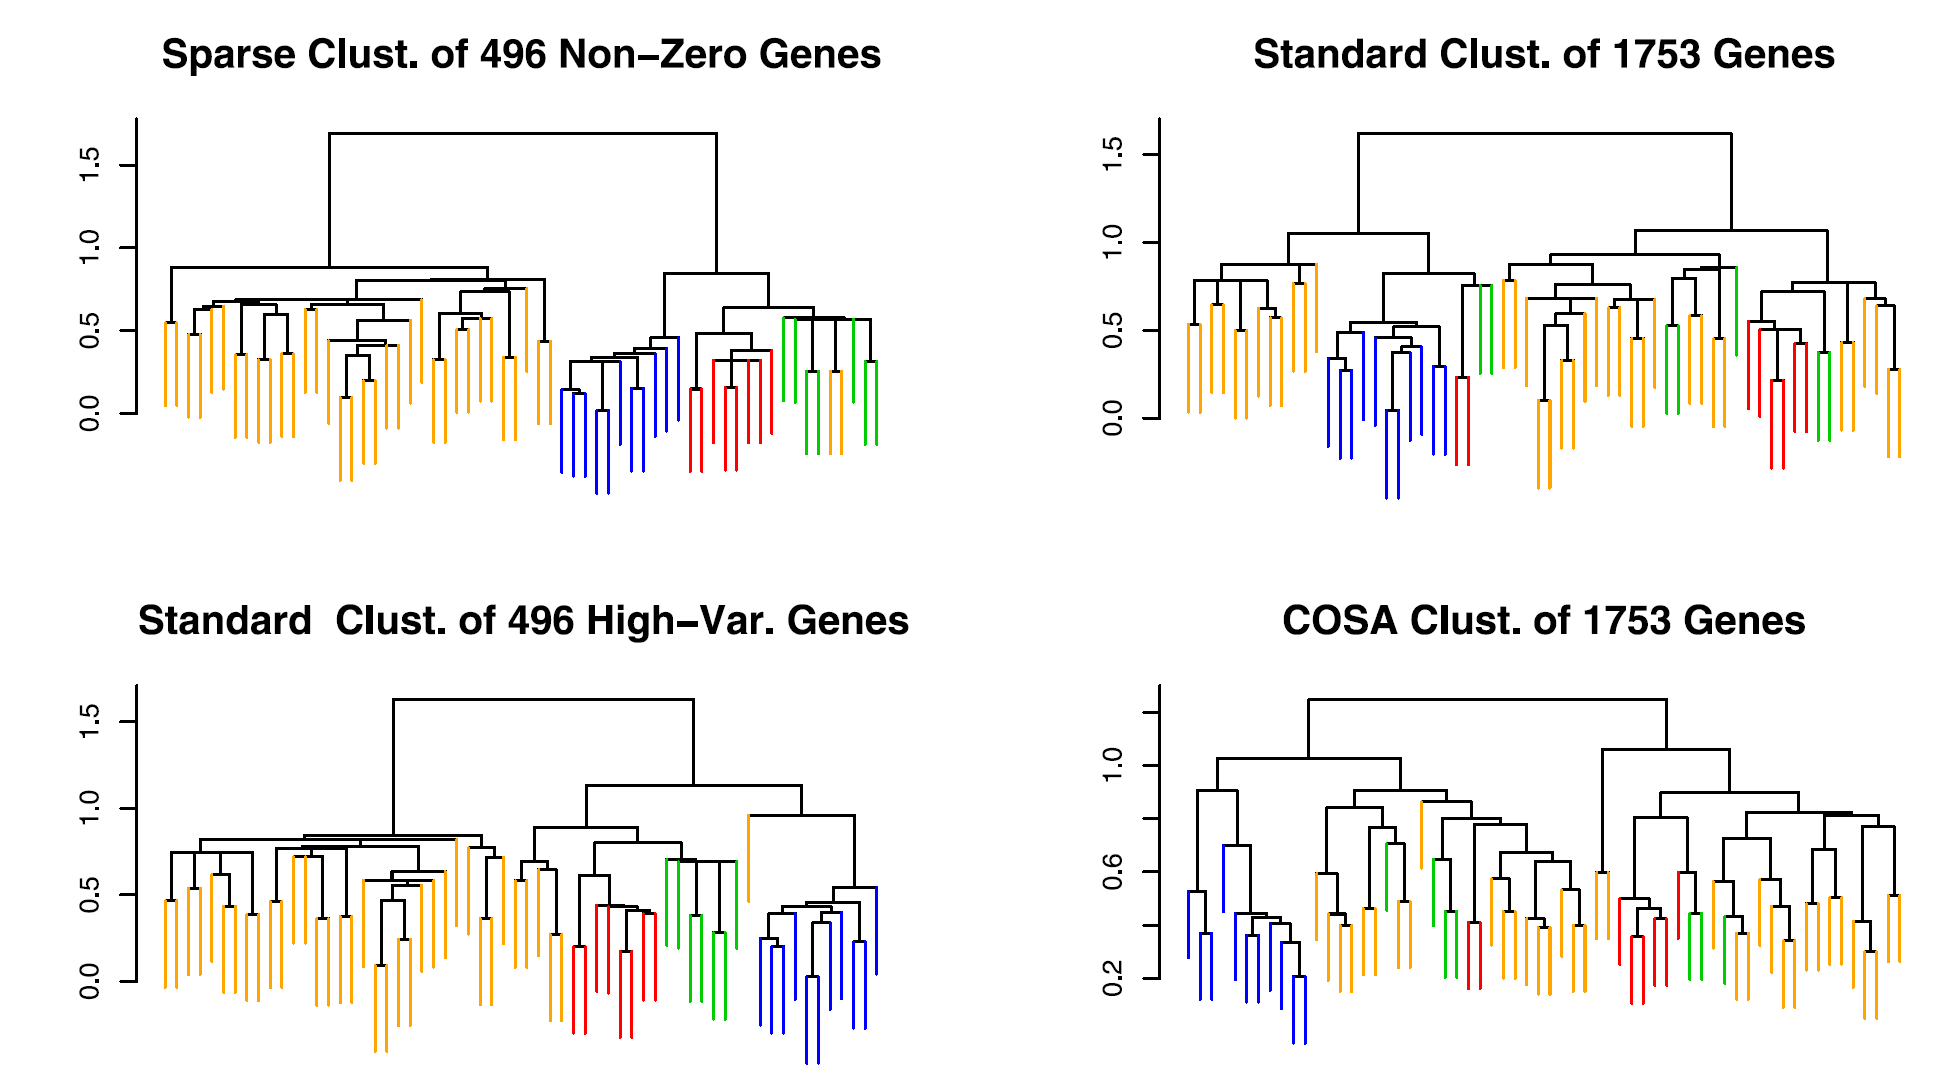
\includegraphics[scale=0.6]{fig7.png}
\end{frame}
\end{document}